\section{Query compiler}
\label{sec:compiler}

Our query compiler transforms a \TheSystem query to target two router backend
targets: (1) the P4 behavioral model~\cite{p4-bmv2} configured by emitting
P4~\cite{p4}, and (2) the Banzai machine model, configured by emitting
Domino code. The emitted code configures a router pipeline,
where each stage is a match-action table~\cite{openflow} or our key-value store.

A preliminary pass of the compiler over the input query converts the query to an
abstract syntax tree (AST) of functional operators. The compiler then
\begin{enumerate}
\item produces router-local ASTs from a global AST
  (\Sec{network-to-router-local});
\item produces \pfs and Domino pipeline configurations from router-level ASTs
  (\Sec{pipeline-layout}); and
\item recognizes linear-in-state aggregation functions, setting up
  auxiliary state for merging later (\Sec{linear-in-state-compilation}).
\end{enumerate}

\begin{figure}[!t]{
\figcodesize
\begin{lstlisting}
def oos_count(count, lastseq, tcpseq, payload_len):
  if lastseq != tcpseq:
    count = count + 1
    emit()
  lastseq = tcpseq + payload_len

tcps    = filter((*\pktlog{}*), proto == TCP
                 and (router == S1 or router == S2));
tslots  = map((*\pktlog{}*), tin/epoch_size, epoch);
joined  = zip(tcps, tslots);
oos     = groupby(joined,
                  [(*\codeftuple{}*), router, epoch],
                  oos_count);
\end{lstlisting}
}
\caption{Running example for \TheSystem compiler (\Sec{compiler}).}
\label{fig:running-example-code}
\end{figure}

\begin{figure}
  \centering
  \[
  \begin{array}{ccc}
    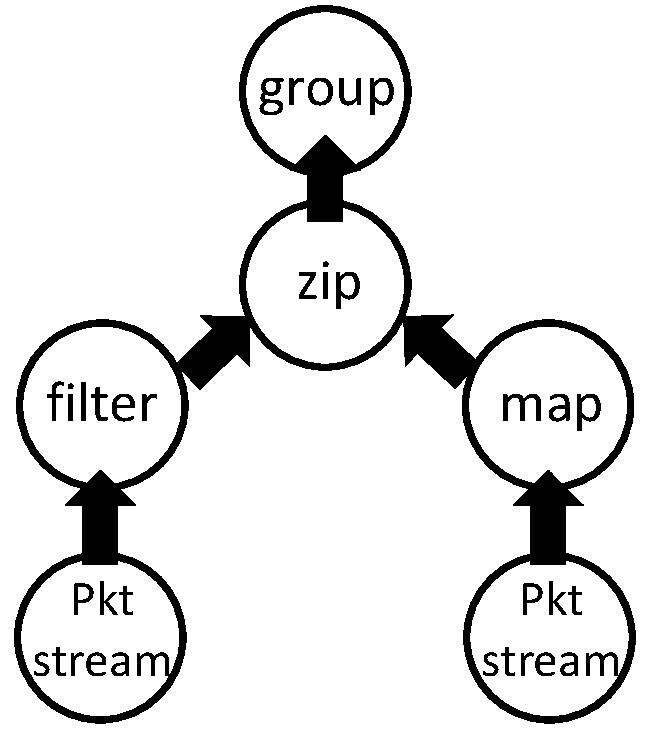
\includegraphics[width=0.31\columnwidth]{pq_running-example-AST.pdf} &
    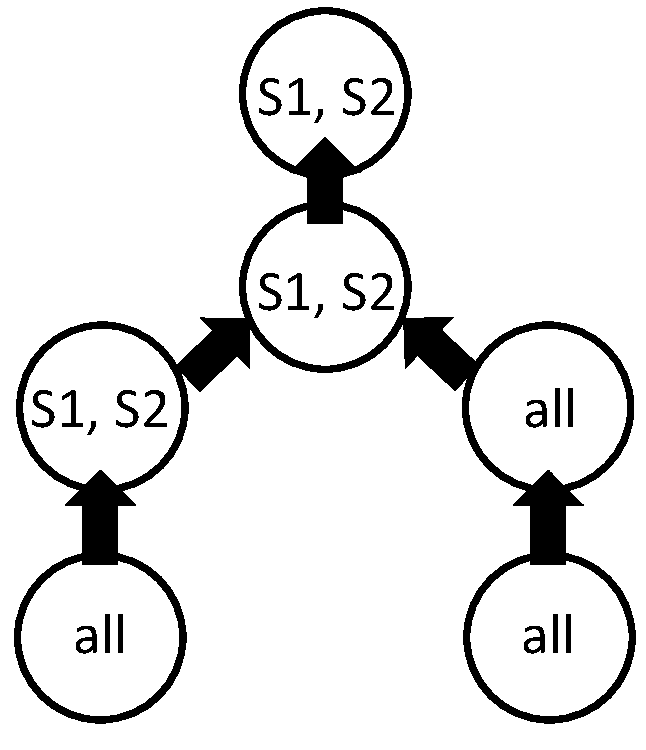
\includegraphics[width=0.31\columnwidth]{pq_running-example-annotated-AST-2.pdf} &
    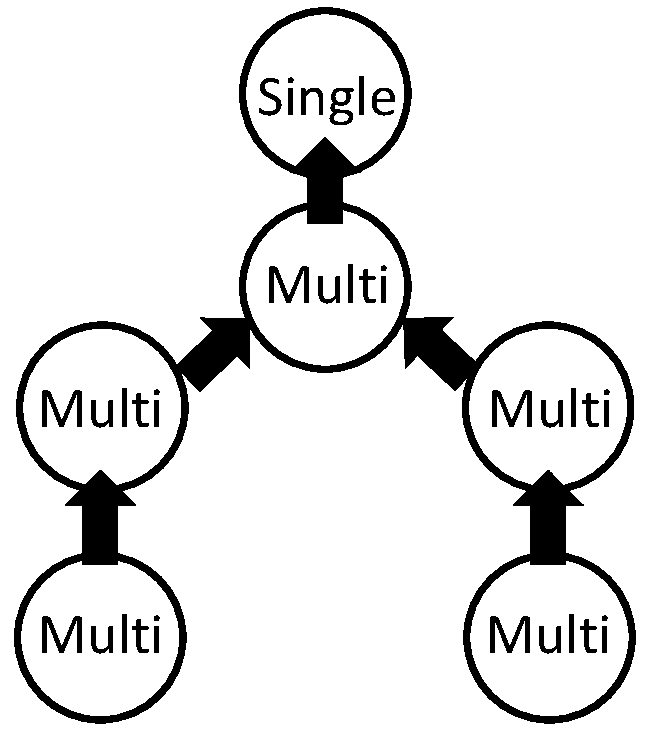
\includegraphics[width=0.31\columnwidth]{pq_running-example-annotated-AST.pdf}
    \\
    \mbox{(a)} & \mbox{(b)} & \mbox{(c)} \\
  \end{array}
  \]
\caption{Compiler manipulations of the Abstract Syntax Tree (AST) for the
  running example (\Sec{compiler}). (a) Operator AST. (b) Stream
  location. (c) Stream type (single/multi-router).}
\label{fig:compiler-ast-manipulations}
\end{figure}

We use the query shown in \Fig{running-example-code} as a running example to
illustrate the details in the compiler. The query counts the number of
out-of-sequence TCP packets over each time epoch, measured at two routers {\ct
  S1} and {\ct S2} in the network.

The compiler begins by parsing the query into an Abstract Syntax Tree (AST) that
is shown in \Fig{compiler-ast-manipulations}(a).

%% four main pieces of compilation
\subsection{Network-wide to switch-local queries}
\label{sec:network-to-switch-local}

The compiler partitions a network-wide query written over all packets at all
queues in the network (\Sec{language}) into switch-local queries to generate
switch-specific configurations. We achieve this in two steps. First, we
determine the {\em stream location}, \ie the set of switches that contribute
tuples to a stream, for the final output stream of query. For instance, the
output stream of a query that filters by switch id $s$ has a stream location
equal to the singleton set $s$. Second, we determine how to partition queries
with aggregation functions written over the entire network into switch-local
queries.
\Anirudh{Mohammad said he didn't get some sentence here. I don't know if it was
the first or second :). NG, can you read the above paragraph once carefully.}


\Para{Determining stream location for the final output stream.} The stream
location of {\ct \pktlog} is the set of all switches in the network. The stream
location of the output of a {\ct filter} is the set of switches implied by the
filter's predicate. Concretely, we evaluate the set of switches contributing
tuples to the output of a {\ct filter} operation through basic syntactic checks
of the form {\ct switch == X} on the {\ct filter} predicate.  We combine switch
sets for boolean combinators ({\ct or} and {\ct and}) inside filter predicates
using set operations (union and intersection respectively). The stream location
of the output
of a {\ct zip} operator is the intersection of the stream locations of the two
inputs.  Stream locations are unchanged by the {\ct map} and {\ct groupby}
operators.

The stream locations for the running example are shown in
\Fig{compiler-ast-manipulations}b. The stream location of {\ct \pktlog} is
the set of all network switches, but is restricted to just {\ct S1} and {\ct
S2} by the {\ct filter} in the query (left branch). This location is then propagated
to the root of the AST through the {\ct zip} operator in the query.

\Para{Partitioning network-wide aggregations.}
As described in \S\ref{sec:language}, we only permit aggregations that satisfy
one of three conditions: they operate independently on each switch, operate
independently on each packet, or are associative and commutative.
We describe below how we
check the first condition, failing which we simply check the last two
conditions syntactically: either the {\ct groupby} aggregates by {\ct uid}
(condition 2) or contains programmer annotations {\ct assoc} and {\ct comm}
(condition 3).

%TODO: The stuff on top still needs to be rewritten ...
To check if an aggregation operates independently on each switch, we label each
AST node with an additional boolean attribute, {\em switch-partitioned},
corresponding to whether the output stream has been partitioned by the switch
at which it appears. Intuitively, if a stream is switch-partitioned, we allow
packet-order-dependent aggregations over multiple packets of that stream;
otherwise, we do not.

Determining and propagating {\em switch-partitioned} through an AST is
straightforward. The base {\ct \pktlog} is not switch-partitioned. The {\ct
  filter} and {\ct zip} operators produce a switch-partitioned stream if their
output only appears at a single switch. The {\ct groupby} produces a
switch-partitioned stream if it aggregates by {\ct switch.} In all other cases,
the operators retain the operands' switch-partitioned attribute.

The switch-partitioned attributes for our running example are shown in
\Fig{compiler-ast-manipulations}c. The {\ct filter} produces output streams at
two switches, hence is not switch-partitioned. The {\ct groupby} aggregates by
{\ct switch} and hence is switch-partitioned. After the partitioning checks have
succeeded, we are left with a set of independent switch-local ASTs corresponding
to each switch location that the AST root operator appears in, \ie {\ct S1, S2}.

\subsection{Query AST to pipeline configuration}
\label{sec:pipeline-layout}

This compiler pass first generates a sequence of operators from the
router-local query AST of \S\ref{sec:network-to-router-local}. This sequence of
operators is then used in the same order to generate a router pipeline
configuration. There are two aspects that require care when constructing a
pipeline structure: (1) the pipeline should respect read-write dependencies
between different streams, and (2) repeated subqueries should not be
re-executed by creating additional pipeline stages.

We generate a sequence of operators through a post-order traversal of the query
AST, which guarantees that the operands of a node are added into the pipeline
before the operator in the node, thereby respecting read-write dependencies.
Further, we deduplicate subquery results from the pipeline to avoid repeating
stages in the final output. For the running example, the algorithm produces the
sequence of operators: {\ct tcps} ({\ct filter}) $\rightarrow$ {\ct tslots}
({\ct map}) $\rightarrow$ {\ct joined} ({\ct zip}) $\rightarrow$ {\ct oos}
({\ct groupby}).

Next, the compiler emits P4 code for a router pipeline from the operator
sequence.  The {\ct filter} and {\ct zip} configuration just involves checking
a predicate and setting a ``valid'' bit on the packet metadata. The {\ct map}
configuration assigns a packet metadata field to the computed expression. The
{\ct groupby} configuration uses a P4 register that is indexed by the
aggregation fields. The state located at a particular register index is updated
through a P4 action representing the aggregation function.

%%We transform
%%\TheSystem aggregation functions into straight-line code consisting of C-style
%%conditional operators through a standard procedure known as
%%if-conversion~\cite{if-conversion}. This allows us to fit the aggregation
%%function into the body of a single P4 action.

To target the Banzai machine model (\S\ref{s:absmachine}), the \TheSystem
compiler emits C-like code fragments for each pipeline stage and then
concatenates these fragments together into a single Domino program. The Domino
compiler then takes this program and compiles it to a pipeline of Banzai atoms.

\subsection{Handling linear-in-state aggregations}
\label{sec:linear-in-state-compilation}

We now consider the problems of detecting if an aggregation function is
linear-in-state and setting up auxiliary state for such linear-in-state
aggregation functions (Figure~\ref{fig:compiler-steps}). Recall that an
aggregation function is linear-in-state if the updates to all state variables
within the aggregation function can be written as $S =
\boldsymbol{A}(\mathbf{p}) \cdot S + \boldsymbol{B}(\mathbf{p})$).  A general
solution to this problem is challenging because the aggregation function can
take varied forms. For instance, the assignment $S = \frac{S^2 - 1}{S -1}$ is
linear-in-state, but detecting that it is linear-in-state needs the compiler to
perform algebraic simplifications.

We take a pragmatic approach and sacrifice completeness, but still cover useful
functions. Specifically, we only detect linear-in-state state updates through
simple syntactic pattern matching in the compiler (\ie without any algebraic
transformations).  Despite these simplifications, the \TheSystem compiler
correctly identifies all the linear-in-state aggregations in
Figure~\ref{fig:example-perf-queries} and targets the multiply-accumulate atom
that we added to the Banzai pipeline.

To describe how linear-in-state detection works, we introduce some terminology.
Recall that an aggregation function takes two arguments (\S\ref{sec:language}):
a list of state variables (\eg a counter) and a list of tuple fields (\eg the
TCP sequence number). We use the term variable in this subsection to refer to
either a state variable or a tuple field. These are the only variables that can
appear within the body of the aggregation function.\footnote{\TheSystem
supports local variables within the function body, but the more general
algorithm is not materially different from the simpler version we present
here.}

\begin{figure}
\centering
% Figure from
% https://docs.google.com/drawings/d/1Y-AC8YxCGkOJsaPILN_Fr1jKed1BKs0UdEab86r9T3g/edit?usp=sharing
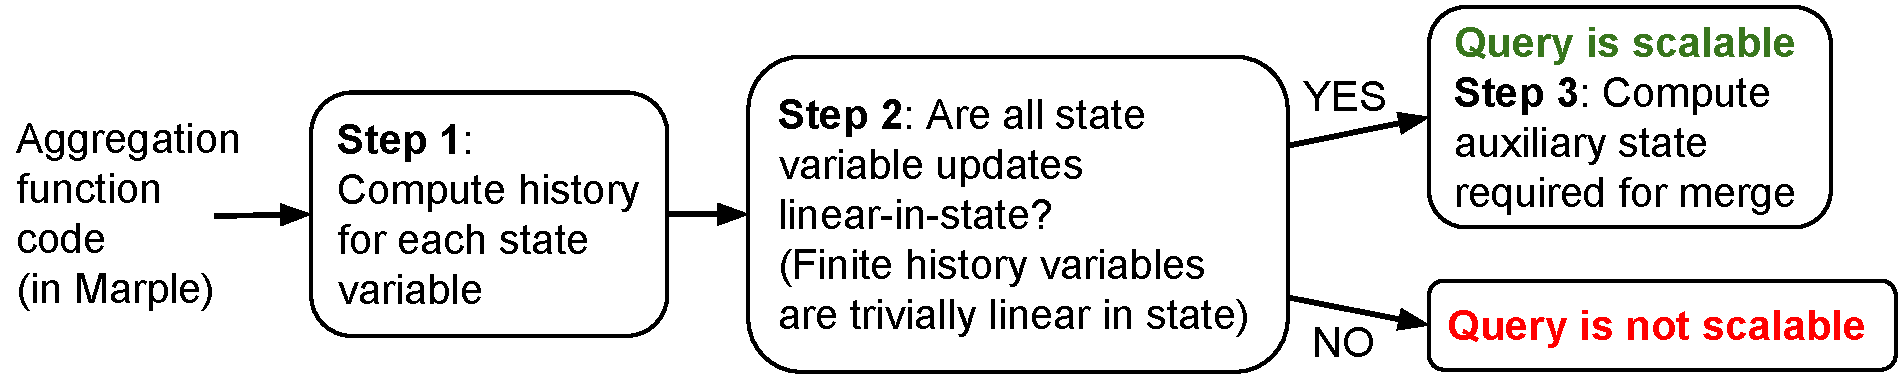
\includegraphics[width=\columnwidth]{pq_compiler-steps.pdf}
\caption{Steps for compiling linear-in-state updates.}
\label{fig:compiler-steps}
\end{figure}

%resume

We carry out a three-step procedure for linear-in-state
detection, summarized in \Fig{compiler-steps}.  First, for each variable in an
aggregation function we assign a {\em history}.  This history tells us how many
previous packets we need to look at to determine a variable's value accurately
(history = 1 means the current packet). For instance, for the value of a byte
counter, we need to look back to the beginning of the packet stream (history =
$\infty$), while for a variable that tracks the last TCP sequence number
we need to only look back to the previous packet (history = 2). Consistent with
the definition of history, constants are assigned a history value of 0, and
variables in the tuple field list are assigned a history of 1. For state
variables, we use \Alg{history} to determine each variable's history.

Second, once each variable has a history, we look at the history of each state
variable $s$. If the history of $s$ is a finite number $k$, then $s$ only
depends on the last $k$ packets and the state update for that variable is
trivially linear-in-state, by setting $A$ to 0 and $B$ to the aggregation
function itself.\footnote{More precisely, the parts of the aggregation function
that update $s$.} If $s$ has an infinite history, we use syntactic pattern
matching to check if the update to $s$ is linear-in-state.

Third, if all state variables have linear-in-state state updates, the
aggregation function is linear-in-state, and we generate the auxiliary state
that permits merging of the aggregation function (\S\ref{sec:aggregation}). If
not, we use the set of stateful instructions developed in Domino~\cite{domino_sigcomm}
to implement the aggregation function. We now describe each of the three steps
in detail.

\Para{Determining history of variables.} To understand \Alg{history}, observe that if all
assignments to a state variable only use variables that have a finite history,
then the state variable itself has a finite history. For instance, in
\Fig{running-example-code}, right after it is assigned, {\ct lastseq} has a history of 1 because it only
depends on the current packet's fields {\ct tcpseq} and {\ct payload\_len}. To
handle branching in the code, \ie {\ct if (predicate) \{...\}} statements, we
generalize this observation. A state variable has finite history if  (1) it 
has finite history in all its assignments in all branches of the program,
and (2) each branching condition {\ct predicate} itself only depends on
variables with a finite history.

Concretely, {\sc computeHistory} (line \ref{line:computeHistoryStart}) assigns each
variable a history corresponding to an upper bound on the number of past
packets that the state variable depends on. We track the history separately for
each branching {\em context}, \ie the sequence of branches enclosing any
statement.\footnote{Currently, \TheSystem forbids multiple {\ctfoot if ...
else} statements at the same nesting level; hence, the enclosing branches
uniquely identify a code path through the function. This restriction is not
fundamental; the more general form can be transformed into this form.} The
algorithm starts with a default large pessimistic history (\ie an approximation
to $\infty$) for each state variable (line \ref{line:curr-hist-init}), and
performs a fixed-point computation (lines
\ref{line:fixed-point}--\ref{line:fixed-point-end}), repeatedly iterating over
the statements in the aggregation function (line
\ref{line:fp-agg-begin}--\ref{line:fp-agg-end}).

For each assignment to a state variable in the aggregation function, the
algorithm updates the history of that state variable in the current branching
context (lines \ref{line:stmt-iteration}--\ref{line:stmt-history-update}). For
each branch in the aggregation function, the algorithm maintains a new
branching context and a history for the branching context itself (lines
\ref{line:encounter-branching}--\ref{line:branch-ctx-update-end}).  At the end
of each iteration, the algorithm increments each variable's history to denote
that the variable is one packet older (line \ref{line:inc}).  The algorithm
returns a conservative history $k$ for each state variable, including possibly
max\_bound (line \ref{line:curr-hist-init}, \Alg{history}) to reflect an
infinite history.

\begin{small}
\begin{algorithm}
  \caption{Determining history of all state variables}
  \label{alg:history}
  \begin{algorithmic}[1]
    \State hist = \{state = \{true: max\_bound\}\} \Comment{Init.
      hist. for all state vars.} \label{line:curr-hist-init}
    \Function{computeHistory}{{\cta fun}}\label{line:computeHistoryStart}
    \While{hist is still changing} \Comment{Run to fixed point.}\label{line:fixed-point}
    \State hist $\gets$ \{\}
    \State ctx $\gets$ true \Comment{Set up outermost context.}
    \State ctxHist $\gets$ 0 \Comment{History value of ctx.}
    \For{stmt in {\cta fun}} \label{line:stmt-iteration} \label{line:fp-agg-begin}
    \If{stmt == {\cta state = expr}}
    \State hist[state][ctx] $\gets$ {\sc getHist}(ctx, expr,
    ctxHist) \label{line:stmt-history-update}
    \ElsIf{stmt == {\cta if predicate}}\label{line:encounter-branching}
    \State save context info (restore on branch exit)\label{line:branch-ctx-update-start}
    \State newCtx $\gets$ ctx \textbf{and} predicate
    \State ctxHist $\gets$ {\sc getHist}(ctx, newCtx, ctxHist)
    \State ctx $\gets$ newCtx\label{line:branch-ctx-update-end}
    \EndIf
    \EndFor \label{line:fp-agg-end}
    \For{ctx, var in hist}\Comment{Make history one pkt older.}
    \State hist[var][ctx] $\gets$ min(hist[var][ctx] + 1, max\_bound)\label{line:inc}
    \EndFor
    \EndWhile \label{line:fixed-point-end}
    \EndFunction
    \Function{getHist}{ctx, {\cta ast}, ctxHist}
    \For{{\cta xi} $\in$ {\sc leafNodes}({\cta ast})}\label{line:used-var-start}
    \State hi = hist[{\cta xi}][ctx]
    \EndFor\label{line:used-var-end}
    \State \textbf{return} max(h1, ... , hn, ctxHist) \label{line:assign-max-hist}
    \EndFunction
  \end{algorithmic}
\end{algorithm}
\end{small}

Now we show precisely how the histories are updated as each statement of the
aggregation function is processed using the helper function {\sc getHist}.
Consider a statement assigning a variable to an expression, {\ct x = expr},
within a branching context {\ct ctx}. Then the history of {\ct x} is the
maximum of the history of the predicates in {\ct ctx} and the history of the
expression {\ct expr}. This is because if either is a function of the last $k$
packets, then {\ct x} is a function of at least the last $k$ packets.  To
determine the history of {\ct expr}, suppose the AST of {\ct expr} contains the
variables {\ct x1, x2, ..., xn} as its leaves. Then, the history of {\ct expr}
is the maximum of the histories of the {\ct xi}.  For example, the history for
{\ct lastseq} after its assignment in {\ct oos\_count} is the maximum of 1
({\ct tcpseq} and {\ct payload\_len} are functions of the current packet), and
0 (for the enclosing outermost context {\ct true}).

%The fixed-point iterations converge because the assigned state histories in a
%context are non-increasing.
%

\Para{Determining if a state variable's update is linear-in-state.} For each
state variable $S$ with an infinite history, we check whether the state updates
are linear-in-state as follows: (1) each update to $S$ is syntactically affine,
\ie $S \gets A \cdot S + B$ with either $A$ or $B$ possibly zero; and (2) $A$,
$B$ and every branch predicate depend on variables with a finite history. This
approach is sound, but incomplete: it misses updates such as $S = \frac{S^2 -
1}{S - 1}$.

\Para{Determining auxiliary state.} For each state variable with a
linear-in-state update, we initialize four pieces of auxiliary state for a
newly inserted key:\footnote{This can happen either when a key first appears or
reappears following an eviction.} (1) a running product $S_A = 1$; (2) a packet
counter $c = 0$; (3) an entry log, consisting of relevant fields from the first
$k$ packets following insertion; and (4) an exit log, consisting of relevant
fields from the last $k$ packets seen so far.  After the counter $c$ crosses
the packet history bound $k$, we update $S_A$ to $A \cdot S_A$ each time $S$ is
updated.\footnote{This stateful update itself can be implemented through a
multiply-accumulate atom.} When the key is evicted, we send $S_A$ along with
the entry and exit logs to the backing store for merging (see Appendix~\ref{app:merge}).

%%\input{compiler-emitting-p4-domino}

